\documentclass[10pt,handout]{beamer}

\usetheme{Madrid}
\usecolortheme{default}

% Base packages
%\usepackage{helvet}
\usepackage{amsthm,graphicx,xcolor,natbib,booktabs,tabularx,mathtools,subcaption}
\usepackage{unicode-math,mathrsfs}
\usepackage{amsmath,amssymb}
\usepackage{tikz,pgfplots}
\usetikzlibrary{arrows.meta, positioning, quotes}

\usepackage[cache=false]{minted}
\renewcommand{\theFancyVerbLine}{\sffamily\textcolor[rgb]{0.5,0.5,1.0}{\scriptsize\oldstylenums{\arabic{FancyVerbLine}}}}
\definecolor{bg}{rgb}{.95,.95,.95}

% Font settings
\renewcommand{\familydefault}{\sfdefault}

% TikZ libraries
\usetikzlibrary{calc,positioning,backgrounds,decorations.pathreplacing}
\pgfplotsset{compat=1.14}

% Colors
\definecolor{deepblue}{RGB}{42,39,155}
\definecolor{lightpink}{RGB}{255,240,240}
\definecolor{lightgreen}{RGB}{240,255,240}
\definecolor{lightyellow}{RGB}{255,255,240}
\definecolor{codegray}{RGB}{245,245,245}
\definecolor{codegreen}{rgb}{0,0.6,0}
\definecolor{codepurple}{rgb}{0.58,0,0.82}

% Beamer settings
\setbeamercolor{title}{fg=white,bg=deepblue}
\setbeamercolor{frametitle}{fg=white,bg=deepblue}
\setbeamercolor{section in head/foot}{fg=white,bg=deepblue}

\setbeamertemplate{footline}[text line]{%
  \parbox{\linewidth}{\vspace*{-8pt}
  %\hfill\href{https://github.com/chang-ye-tu/fin}{https://github.com/chang-ye-tu/fin}
    \hfill
   \insertframenumber~/ \inserttotalframenumber}}
\setbeamertemplate{navigation symbols}{}%[only frame symbol]

\definecolor{foo}{rgb}{.2,.2,.7}
\AtBeginSection[]{
  \begin{frame}
  \vfill
  \centering
  \begin{beamercolorbox}[sep=8pt,center,shadow=true,rounded=true]{section page}
    \usebeamerfont{title}%
    {\color{foo} \insertsectionhead}\par%
  \end{beamercolorbox}
  \vfill
  \end{frame}
}

% https://tex.stackexchange.com/questions/30423/bibliography-in-beamer
\setbeamertemplate{bibliography entry title}{}
\setbeamertemplate{bibliography entry location}{}
\setbeamertemplate{bibliography entry note}{}

\usepackage{dsfont} % indicator function \mathds{1}
\DeclareMathOperator\indc{\mathds{1}}
\newcommand{\ds}{\displaystyle}
\newcommand{\ie}{\;\Longrightarrow\;}
\newcommand{\ifff}{\;\Longleftrightarrow\;}
\newcommand{\mi}{\mathrm{i}}
\DeclareMathOperator*{\dom}{dom}
\DeclareMathOperator*{\codom}{codom}
\DeclareMathOperator*{\ran}{ran}
\newcommand{\floor}[1]{\lfloor #1 \rfloor}
\newcommand{\ceil}[1]{\lceil #1 \rceil}
\newcommand{\Set}[2]{\big\{ \ #1\ \big|\ #2\ \big\}}
\newcommand{\pdiff}[2]{\frac{\partial\hfil#1\hfil}{\partial #2}}
\newcommand{\vx}{\symbfup{x}}
\newcommand{\vd}{\symbfup{d}}
\newcommand{\vg}{\symbfup{g}}
\newcommand{\vH}{\symbfup{H}}
\newcommand{\va}{\symbfup{a}}
\newcommand{\vb}{\symbfup{b}}
\newcommand{\vbb}{\symbfup{\beta}}
\newcommand{\vS}{\symbfup{S}}
\newcommand{\vR}{\symbfup{R}}
\newcommand{\vV}{\symbfup{V}}
\newcommand{\ve}{\symbfup{e}}
\newcommand{\vr}{\symbfup{r}}
\newcommand{\vZero}{\symbfup{0}}

\DeclareMathOperator\prb{{\sf P}}
\DeclareMathOperator\expc{{\sf E}}
\DeclareMathOperator\var{var}
\DeclareMathOperator\cov{cov}
\DeclareMathOperator\cor{cor}
\DeclareMathOperator*{\argmax}{\arg\!\max}
\DeclareMathOperator*{\argmin}{\arg\!\min}
\DeclareMathOperator*{\im}{Im}
\DeclareMathOperator*{\re}{Re}
\DeclareMathOperator*{\conv}{conv}
\DeclareMathOperator*{\proj}{proj}
\DeclareMathOperator*{\tr}{tr}
\DeclareMathOperator*{\diag}{diag}
\DeclareMathOperator*{\epi}{epi}
\DeclareMathOperator*{\dist}{dist}
\DeclareMathOperator*{\inte}{int}
\DeclareMathOperator*{\relint}{relint}

\theoremstyle{definition}
\newtheorem*{dfn}{Definition}
\newtheorem*{prp}{Property}
\newtheorem*{thm}{Theorem}
\newtheorem*{ex}{Example}
\newtheorem*{prob}{Problem}
\newtheorem*{sol}{Solution}
\newtheorem*{prf}{Proof}
\usepackage{nicefrac}
\usepackage{multicol}

\newcommand\scalemath[2]{\scalebox{#1}{\mbox{\ensuremath{\displaystyle #2}}}}

\title{Options \& Derivatives}
\author{}
\date{}

\begin{document}

\begin{frame}
\titlepage
\end{frame}

%\subsection*{Outline}
%\begin{frame}
%  \tableofcontents
%\end{frame}

\begin{frame}{The One Period Model}
  \begin{itemize}
    \item time $t$: $t=0, 1$ 
    \item (deterministic) bond $B_t$: $\ds B_0 = 1,\;B_1 = 1 + R$
    \item (stochastic) stock $S_t$: $\ds S_0 = s > 0, \; S_1 = \begin{cases} s\cdot u & \text{with prob. } p_u\\ s\cdot d & \text{with prob. } p_d \end{cases} \equiv s\,Z:\;$ $u > d$, $p_u + p_d = 1$.
    \item The value $V_t^h$ of the portfolio $h=(x, y),\,x, y\in\mathbb{R}$ at time $t$: $\ds V_t^h = x\,B_t + y\,S_t$ --- $\ds V_0^h = x + y\,s,\; V_1^h = x(1 + R) + y\,s\,Z$
    \item Arbitrage portfolio $h$: $V_0^h=0$, $V_1^h>0$ with prob. $1$.
  \end{itemize}
  \begin{figure}[!htbp]
    \centering
    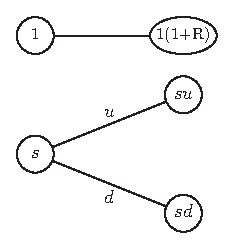
\includegraphics[scale=0.9,page=1]{fig/note08/bjork.pdf}
    \caption{Asset Dynamics of One Period Model.}
    \label{fig:bn1}
  \end{figure}
\end{frame}

\begin{frame}{Portfolios and Arbitrage I}
  \begin{thm}
    The one period model is arbitrage free $\ifff$ $\ds u\geqslant 1+R \geqslant d$.
  \end{thm}
  \begin{prf}
    ($\Longrightarrow$)
    \begin{itemize}
      \item Suppose $u\geqslant 1+R \geqslant d$ does not hold, then $1 + R > u$ or $d > 1 + R$.
      \item If $1 + R > u$, then $s(1 + R) > s\,u$ and a priori $s(1+R) > s\,d$.
      \item Consider $h = (s, -1)$, then $V_0^h = s\cdot 1 + (-1)\cdot s = 0$, $V_1^h = s(1 + R) - s\cdot Z >0$, an arbitrage.
      \item If $d > 1 + R$, then $s\,d > s(1 + R)$ and a priori $s\,u > s(1 + R)$.
      \item Consider $h = (-s, 1)$, then $V_0^h = (-s)\cdot 1 + 1\cdot s = 0$, $V_1^h = -s(1 + R) + s\cdot Z > 0$, an arbitrage.
    \end{itemize}
  \end{prf}
\end{frame}
\begin{frame}{Portfolios and Arbitrage II}
  \begin{thm}
    The one period model is arbitrage free $\ifff$ $\ds u\geqslant 1+R \geqslant d$.
  \end{thm}
  \begin{prf}
    ($\Longleftarrow$)
    \begin{itemize}
      \item Arbitrage $h = (x, y)$: $V_0^h = 0$.
      \item $ x + s\cdot y = 0\ie x= -s\cdot y$. 
      \item $\ds V_1^h = \begin{cases}y\,s\big(u - (1 + R)\big),&\; Z=u \\ y\,s\big(d - (1 + R)\big),&\; Z=d\end{cases}$
      \item If $y > 0$: from $\ds V_1^h > 0$ $\ie$ $u > 1 + R$ and $d > 1 + R$; a contradiction.
      \item If $y < 0$: from $\ds V_1^h > 0$ $\ie$ $u < 1 + R$ and $d < 1 + R$; a contradiction.
    \end{itemize}
  \end{prf}
\end{frame}

%\begin{thm}
%  $\ds \text{ No arbitrage }\ifff u\geqslant 1+R \geqslant d$
%\end{thm}

\begin{frame}{Risk-Neutral / Martingale Measure and Probabilities}
  \begin{itemize}
    \item Observation: $u\geqslant 1+R \geqslant d$ $\ie$ $1 + R$ is a convex combination of $u$ and $d$  
    \item $\ds\exists\,q_u, q_d \geqslant 0,\,\,q_u+q_d = 1\;\text{ s.t. }\; 1 + R = q_u\cdot u + q_d\cdot d$
    \item Define a new probability measure $Q$ and the associated expectation $\expc^Q$ s.t. 
      \begin{align*}
        &Q(Z = u) = q_u,\quad Q(Z = d) = q_d \\
        &\frac{1}{1+R}\expc^Q S_1 = \frac{1}{1+R}(q_u\cdot s\,u + q_d\cdot s\,d) = \frac{1}{1+R}\cdot s(1+R) = s
      \end{align*}
  \end{itemize}
  \begin{dfn}
    \begin{itemize}
      \item \textbf{Risk-Neutral / Martingale Measure}: A measure $Q$ satisfies $\ds S_0 = \frac{1}{1+R}\expc^Q S_1$.
      \item \textbf{Martingale Probabilities}: $\ds q_u = \frac{(1+R)-d}{u-d}, \;q_d = \frac{u-(1+R)}{u-d}$
    \end{itemize}
  \end{dfn}
\end{frame}

\begin{frame}{Contingent Claims I}
  \begin{dfn}
    \begin{itemize}
      \item A \textbf{contingent claim} $X$ is of the form $X=\Phi(Z)$
      \item Stochastic $Z$ with \textbf{contract function} $\Phi(\cdot)$
      \item \textbf{Price} of $X$ at time $t$: $\Pi(t; X)$
    \end{itemize}
  \end{dfn}
  \begin{figure}[!htbp]
    \centering
    \includegraphics[scale=.9,page=2]{fig/note08/bjork.pdf}
    \caption{The Contingent Claim.}
    \label{fig:bn2}
  \end{figure}
\end{frame}

\begin{frame}{Contingent Claims II}
  \begin{example}[European Call Option with Strike $K$]
    Assume $s\, u > K > s\, d$. At $t=1$, 
    \begin{itemize}
      \item Exercise the option if $S_1 > K$.
        \begin{itemize}
          \item Pay $K$ to get the stock and sell it at $s\,u$, thus making net profit $s\,u-K$.
        \end{itemize}
      \item Do nothing if $S_1 < K$.
    \end{itemize}
    \begin{align*}
      X = \begin{cases}s\,u - K, & Z=u \\ 0,  & Z=d\end{cases}, \quad\begin{cases}\Phi(u) = s\, u - K \\ \Phi(d) = 0\end{cases}
    \end{align*}
  \end{example}
  \begin{dfn}
    \begin{itemize}
      \item A contingent claim $X$ is said to be \textbf{reachable} if there exists a portfolio $h$ such that $V_1^h = X$ with probability 1; this portfolio $h$ is called a \textbf{hedging} or \textbf{replicating} portfolio. 
      \item If all claims can be replicated we say the market is \textbf{complete}.
    \end{itemize}
  \end{dfn}
\end{frame}

\begin{frame}{Contingent Claims III}
\begin{thm}[Pricing Principle]
  If a claim $X$ is reachable with replicating portfolio $h$, then the ``reasonable'' price of $X$ is given by $\ds\Pi(t; X) = V_t^h, \; t=0, 1.$
\end{thm}

\begin{thm}
  An arbitrage free one period model is complete.
\end{thm}

\begin{prf}
  Fixed any $\Phi(\cdot)$, show that $\exists\,h=(x, y)$ s.t.
  \begin{align*}
    V_1^h = \begin{cases}\Phi(u)\quad Z=u,\\ \Phi(d)\quad Z=d.\end{cases}\!\!\!\!\Longrightarrow x(1+R) + y\,s\,u = \Phi(u), \; x(1+R) + y\,s\,d = \Phi(d).
  \end{align*}
  Solve for $x, y$: $\ds x = \frac{1}{1+R}\,\frac{u\Phi(d)-d\,\Phi(u)}{u-d},\quad y = \frac{1}{s}\,\frac{\Phi(u)-\Phi(d)}{u-d}$.
\end{prf}
\end{frame}

\begin{frame}{Risk Neutral Valuation}
  \begin{itemize}
    \item From Pricing Principle ($\Pi(t; X) = V_t^h,\, t=0,1$)
      \begin{align*}
        \Pi(0; X) &= V_0^h = x + s\,y \\
                  &= \frac{1}{1+R}\cdot\frac{u\Phi(d)-d\,\Phi(u)}{u-d} + s\cdot\frac{1}{s}\cdot\frac{\Phi(u)-\Phi(d)}{u-d} \\
                  &= \frac{1}{1+R}\left\{\frac{(1+R)-d}{u-d}\,\Phi(u) + \frac{u-(1+R)}{u-d}\,\Phi(d)\right\}\\
                  &= \frac{1}{1+R}\left\{q_u\,\Phi(u) + q_d\,\Phi(d)\right\} \equiv \frac{1}{1+R}\expc^Q X
      \end{align*}
  \end{itemize}
  \begin{thm}[The Risk Neutral Valuation Principle]
    If the one period binomial model is arbitrage-free, then the price of $X$ is $\ds\Pi(0; X) = \frac{1}{1+R}\expc^Q X$.
  \end{thm}
\end{frame}

\begin{frame}{The Multiperiod Model}
  \begin{itemize}
    \item time $t$: $t=0, 1, 2, \ldots, T$ 
    \item (deterministic) bond $B_t$ with $\ds B_0 = 1,\; B_{n+1} = (1 + R)B_n$
    \item (stochastic) stock $S_t$ with $\ds S_0 = s > 0,\; S_{n+1} = Z_n\,S_n$ where $Z_0, Z_1, Z_2,\ldots, Z_{T-1}$ are iid with $\ds\prb(Z_n=u) = p_u,\;\prb(Z_n=d) = p_d$
  \end{itemize}
  \begin{figure}[!htbp]
    \centering
    \includegraphics[scale=.75,page=3]{fig/note08/bjork.pdf}
    \vspace{-3mm}
    \caption{Asset Dynamics of Multiperiod Model: ``Recombining'' Tree.}
    \label{fig:bn3}
  \end{figure}
\end{frame}

\begin{frame}{Portfolios and Arbitrage}
\begin{dfn}
  The portfolio $h_t \equiv (x_t, y_t)$; The value $V_t^{h_t}$ of portfolio $h_t$ at time $t$ is $\ds V_t^{h_t} = x_t\,B_t + y_t\,S_t$.
\end{dfn}
\begin{itemize}
  \item Hereafter we write $V_t^h$ instead of the cumbersome $V_t^{h_t}$. 
  \item $x_t$ is the amount which we invest in the bank at time $t-1$ and keep until $t$.
\end{itemize}
\begin{dfn}
  Self-financing portfolio $h_t=(x_t, y_t)$: $\ds x_t\,(1 + R) + y_t\,S_t = x_{t+1} + y_{t+1}\,S_t,\quad\forall t = 0, 1, \ldots, T-1.$
\end{dfn}
\end{frame}

\begin{frame}{Contingent Claims}
\begin{dfn}
  \begin{itemize}
    \item Arbitrage: there exists a self-financing portfolio $h_t$ with $\ds V_0^h = 0$, $\prb(V_T^h\geqslant 0) = 1$, $\ds\prb(V_T^h>0) > 0$.
    \item A contingent claim $X$ is said to be \textbf{reachable} if there exists a self-financing portfolio $h$ such that $V_T^h = X$ with probability 1; this portfolio $h$ is called a \textbf{hedging} or \textbf{replicating} portfolio. 
    \item If all claims can be replicated we say the market is \textbf{complete}. 
  \end{itemize}
\end{dfn}

\begin{thm}[Pricing Principle]
  If a claim $X$ is reachable with replicating (and self-financing) portfolio $h$, then the ``reasonable'' price process of $X$ is given by $\ds \Pi(t; X) = V_t^h, \; t=0, 1, 2, \ldots T$.
\end{thm}

\begin{thm}
  An arbitrage-free multiperiod model is complete.
\end{thm}
\end{frame}
  
\begin{frame}
  \begin{thm}[Binomial Algorithms]
    \begin{itemize}
      \item Given a contingent claim $X=\Phi(S_T)$; let $V_t(k)$ denotes the value of the replicating portfolio at node $(t, k)$, then $V_t(k)$ is computed recursively by 
        \begin{align*}
          V_T(k) &= \Phi(s\,u^k\,d^{T-k}) \\
          V_t(k) &= \frac{1}{1+R}\left\{q_u\,V_{t+1}(k+1) + q_d\,V_{t+1}(k)\right\}
        \end{align*}
      \item The martingale probabilities $q_u, q_d$ are $\ds q_u = \frac{(1+R)-d}{u-d}$, $\ds q_d = \frac{u-(1+R)}{u-d}$
      \item The replicating portfolio $h_t = (x_t, y_t)$ is \vspace{-3mm}
        \begin{align*}
          x_t(k) = \frac{1}{1+R}\,\frac{u\,V_t(k)-d\,V_t(k+1)}{u-d}, \quad y_t(k) = \frac{1}{S_{t-1}}\,\frac{V_t(k+1)-V_t(k)}{u-d}
        \end{align*}
      \item The arbitrage-free price of a contingent claim $X$ at $t=0$ is \vspace{-3mm} 
    \begin{align*}
      \Pi(0;X) = \frac{1}{(1 + R)^T}\expc^Q X = \frac{1}{(1 + R)^T}\cdot\sum_{k=0}^T\binom{T}{k}q_u^k\,q_d^{T-k}\Phi(s\,u^k\,d^{T-k})
    \end{align*}
    \end{itemize}
  \end{thm}
\end{frame}

\begin{frame}
  \begin{example}
    Given $T=3, S_0=80, K=80, u=1.5, d=0.5, p_u=0.6, p_d=0.4, R=0$, compute the European call option price and the replicating portfolio of each node.
  \end{example}
  \begin{figure}
    \centering
    \includegraphics[scale=.9,page=4]{fig/note08/bjork.pdf}
    \caption{Asset Dynamics of the Example.}
  \end{figure}  
\end{frame}

\begin{frame}
  \begin{figure}[!htbp]
    \centering
    \includegraphics[scale=1,page=5]{fig/note08/bjork.pdf}
    \caption{Payoff at the End of Terms.}
  \end{figure}
\end{frame}

\begin{frame}
  \begin{figure}[!htbp]
    \centering
    \includegraphics[scale=1,page=7]{fig/note08/bjork.pdf}
    \caption{Iterated Computation of $\ds\Pi(t;X):\;$ $\ds\Pi(t-1; X)\equiv\frac{1}{1+R}\expc^Q\{\Pi(t; X)\}$.} %$\;\ds = \frac{1}{1+R}\left\{q_u\Phi(u) + q_d\Phi(d)\right\}$}
  \end{figure}
\end{frame}

\begin{frame}
  \begin{figure}[!htbp]
    \centering
    \includegraphics[scale=1,page=9]{fig/note08/bjork.pdf}
    \caption{The Completed $\Pi(t; X)$.} 
  \end{figure}
\end{frame}

\begin{frame}
  \begin{figure}[!htbp]
    \centering
    \includegraphics[scale=1.05,page=10]{fig/note08/bjork.pdf}
    \caption{Replicating $h_t=(x_t, y_t):\;$ $x_t(k) = \frac{1}{1+R}\,\frac{u\,V_t(k)-d\,V_t(k+1)}{u-d}$, $y_t(k) = \frac{1}{S_{t-1}}\,\frac{V_t(k+1)-V_t(k)}{u-d}$}
  \end{figure}
\end{frame}

\begin{frame}
  \frametitle{Algorithmic Considerations}
    \begin{align*}
      \Pi(0;X)=\frac{1}{(1 + R)^T}\cdot\sum_{k=0}^T\binom{T}{k}q_u^k\,q_d^{T-k}\Phi(s\,u^k\,d^{T-k})
    \end{align*}
    For big $T$ the formula can't be directly used because of the binomial coefficient
    \begin{align*}
      V_T(k) = \Phi(s\,u^k\,d^{T-k}), \quad V_t(k) = \frac{1}{1+R}\left\{q_u\,V_{t+1}(k+1) + q_d\,V_{t+1}(k)\right\}
    \end{align*}
  \begin{figure}
    \includegraphics[width=.45\textwidth,page=2]{fig/note08/gilli.pdf}
    \includegraphics[width=.45\textwidth,page=3]{fig/note08/gilli.pdf}
    %\caption{Vector Update} 
  \end{figure}
\end{frame}

\begin{frame}[fragile]{Python Code Illustration: Common Parts}
  \begin{minted}{python}
  import numpy as np
  
  S0 = 80; r = 0; K = 80; u = 1.5; d = 0.5; 
  q = (1 - d) / (u - d); M = 3; 
  df = 1     # discount factor per time interval
  # exhibit stock paths
  S = np.zeros((M + 1, M + 1), dtype=np.float)  
  S[0, 0] = S0
  for j in range(1, M + 1, 1):
      for i in range(j + 1):
          S[i, j] = S[0, 0] * (u ** (j - i)) * (d ** i)
  \end{minted}
\end{frame}
  
\begin{frame}[fragile]{Python Codes: Traditional Loops}
  \begin{minted}[fontsize=\small]{python}
  iv = np.zeros((M + 1, M + 1), dtype=np.float); z = 0  # inner values
  for j in range(0, M + 1, 1):
      for i in range(z + 1):
          iv[i, j] = round(max(S[i, j] - K, 0), 8)
      z += 1
  
  pv = np.zeros((M + 1, M + 1), dtype=np.float)         # present values
  pv[:, M] = iv[:, M]
  z = M + 1
  for j in range(M - 1, -1, -1):
      z -= 1
      for i in range(z):
          pv[i, j] = (q * pv[i, j + 1] + (1 - q) * pv[i + 1, j + 1]) * df
  \end{minted}
\end{frame}

\begin{frame}{Python Codes: Vectorized Loops}
  \inputminted[fontsize=\footnotesize,linenos=true]{python}{fig/note08/binomial_vec.py}
\end{frame}

\begin{frame}{Option Pricing in Continuous Time}
  \begin{itemize}
    \item Option pricing in discrete time: for contract $X$ 
      \begin{align*}
        \Pi(0;\,X) = \frac{1}{(1 + R)^T}\expc^Q{X_T}
      \end{align*}
    \item Discretize each interval further into $m$ sections, then the compounding factor $(1 + R)^T$ becomes $(1 + \frac{R}m)^{mT}$
    \item Let $m\to\infty$ (continuous time), $(1 + \frac{R}m)^{mT}\to e^{RT}$
    \item So option pricing in continuous time: for contract $X$ 
      \begin{align*}
        \Pi(0;\,X) = e^{-RT}\expc^Q{X_T}
      \end{align*}
    \item Hereafter $r$, instead of $R$, is the underlying interest rate 
  \end{itemize}
\end{frame}

\begin{frame}{Option Pricing: The Black-Scholes Formula I}
  \begin{itemize}
    \item Under the risk-neutral probability measure $Q$, the stock $S$ evolves as $S(t) = S(0)\,\exp\big\{\big(r - \delta - \frac{\sigma^2}{2}\big)t + \sigma\sqrt{t}Z\big\}$, where $Z\sim N(0, 1)$.
    \item For the European call option with strike $K$, the contract is $X(t) = \max\{S(t) - K,\,0\} \equiv (S(t) - K)_+$.
    \item So the price of the call option at $t = 0$ is
      \begin{align*}
        \Pi_c(0;\,X) &= e^{-rT}\expc^Q\{X(T)\} = e^{-rT}\expc^Q\{(S(T) - K)_+\} \\ 
        &= e^{-rT}\expc^Q\{(S(T) - K)_+\,|\, S(T) > K\} \prb^Q\{S(T) > K\} \\
        &\qquad+ e^{-rT}\underbrace{\expc^Q\{(S(T) - K)_+\,|\, S(T) < K\}}_{ = 0} \prb^Q\{S(T) < K\} \\
        &= e^{-rT}\expc^Q\{(S(T) - K)_+\,|\, S(T) > K\} \prb^Q\{S(T) > K\} \\
        &= e^{-rT}\expc^Q\{S(T) - K\,|\, S(T) > K\} \prb^Q\{S(T) > K\} \\ 
        &= e^{-rT}\big(\expc^Q\{S(T)\,|\, S(T) > K\} - K\big)\prb^Q\{S(T) > K\} 
      \end{align*}
  \end{itemize}
\end{frame}

\begin{frame}{Option Pricing: The Black-Scholes Formula II}
  \begin{itemize} 
    \item As $S(T) = S(0)\,\exp\big\{\big(r - \delta - \frac{\sigma^2}{2}\big)T + \sigma\sqrt{T}Z\big\}$, evaluate $\prb^Q\{S(T) > K\}$ and $\expc^Q\{S(T)\,|\, S(T) > K\}$
    \item Let $\Phi(\cdot)$ be the CDF of $N(0, 1)$, then \vspace{-3mm}
      \begin{align*}
        \prb^Q\{S(T) > K\} &= \prb^Q\!\Big\{S(0)\,\exp\Big\{\Big(r - \delta - \frac{\sigma^2}{2}\Big)T + \sigma\sqrt{T}Z\Big\} > K\Big\} \\ 
        &=\prb^Q\!\Big\{\exp\Big\{\Big(r - \delta - \frac{\sigma^2}{2}\Big)T + \sigma\sqrt{T}Z\Big\} > \frac{K}{S(0)}\Big\} \\
        &=\prb^Q\!\Big\{\Big(r - \delta - \frac{\sigma^2}{2}\Big)T + \sigma\sqrt{T}Z > \ln\frac{K}{S(0)}\Big\} \\
%        &=\prb^Q\!\Big\{\sigma\sqrt{T}Z > \ln\frac{K}{S(0)} - \Big(r - \delta - \frac{\sigma^2}{2}\Big)T\Big\} \\
        &=\prb^Q\!\bigg\{Z > \frac{\ln\frac{K}{S(0)} - \big(r - \delta - \frac{\sigma^2}{2}\big)T}{\sigma\sqrt{T}}\bigg\} \\
        &=1 - \Phi\bigg(\frac{\ln\frac{K}{S(0)} - \big(r - \delta - \frac{\sigma^2}{2}\big)T}{\sigma\sqrt{T}}\bigg) \\
        &=\Phi\bigg(\frac{\ln\frac{S(0)}{K} + \big(r - \delta - \frac{\sigma^2}{2}\big)T}{\sigma\sqrt{T}}\bigg) \equiv \Phi(d_2)
      \end{align*}
  \end{itemize}
\end{frame}

\begin{frame}{Option Pricing: The Black-Scholes Formula III}
  \begin{itemize} 
    \item Define $\ds d_2 = \frac{\ln\frac{S(0)}{K} + \big(r - \delta - \frac{\sigma^2}{2}\big)T}{\sigma\sqrt{T}}$, $\ds d_1$ $=$ $\ds\frac{\ln\frac{S(0)}{K} + \big(r - \delta + \frac{\sigma^2}{2}\big)T}{\sigma\sqrt{T}}$ $=$ $d_2 + \sigma\sqrt{T}$; $\;\ds\expc^Q\{S(T)\,|\, S(T) > K\} = \frac{\expc^Q\big\{S(T)\indc_{\{S(T) > K\}}\big\}}{\prb^Q\{S(T) > K\}}$ and \vspace{-2mm}
      \begin{align*}
        \expc^Q\big\{S(T)\indc_{\{S(T) > K\}}\big\} &= \expc^Q\big\{S(T)\indc_{\{Z > -d_2\}}\big\} \\
        &= \int_{-d_2}^\infty S(0)\,e^{\big(r - \delta - \frac{\sigma^2}{2}\big)T + \sigma\sqrt{T}z}\cdot\frac{1}{\sqrt{2\pi}}e^{-\frac{1}{2}z^2}\,\mathrm{d}z \\
        &= S(0)\,e^{(r - \delta)T}\int_{-d_2}^\infty \frac{1}{\sqrt{2\pi}}e^{-\frac{1}{2}z^2 + \sigma\sqrt{T}z - \frac{1}{2}\sigma^2 T}\,\mathrm{d}z \\
        &= S(0)\,e^{(r - \delta)T}\int_{-d_2}^\infty \frac{1}{\sqrt{2\pi}}e^{-\frac{1}{2}(z - \sigma\sqrt{T})^2}\,\mathrm{d}z \\
        &= S(0)\,e^{(r - \delta)T}\int_{-d_2-\sigma\sqrt{T}}^\infty \frac{1}{\sqrt{2\pi}}e^{-\frac{1}{2}z^2}\,\mathrm{d}z \\
        &= S(0)\,e^{(r - \delta)T}\int_{-d_1}^\infty \frac{1}{\sqrt{2\pi}}e^{-\frac{1}{2}z^2}\,\mathrm{d}z = S(0)\,e^{(r - \delta)T}\Phi(d_1)
      \end{align*} 
  \end{itemize}
\end{frame}

\begin{frame}{Option Pricing: The Black-Scholes Formula IV}
  \begin{itemize}
    \item The price of the call option with strike $K$ at $t = 0$ is
      \begin{align*}
        \Pi_c(0;\,X) &= e^{-rT}\big(\expc^Q\{S(T)\,|\, S(T) > K\} - K\big)\prb^Q\{S(T) > K\} \\
        &= e^{-rT}\expc^Q\big\{S(T)\indc_{\{S(T) > K\}}\big\} - Ke^{-rT}\prb^Q\{S(T) > K\} \\
        &= e^{-rT}S(0)\,e^{(r - \delta)T}\Phi(d_1) - Ke^{-rT}\Phi(d_2) \\
        &= S(0)\,e^{-\delta T}\Phi(d_1) - Ke^{-rT}\Phi(d_2)
      \end{align*}
    \item Note that 
      \begin{align*}
        (S(T) - K)_+ - (K - S(T))_+ &= \max\{S(T) - K, 0\} - \max\{K - S(T), 0\} \\
        &= \max\{S(T) - K, 0\} + \min\{S(T) - K, 0\} \\ &= S(T) - K
      \end{align*}
    \item Let the price of the put option with strike $K$ at $t = 0$ be $\Pi_p(0;\,X)$, then
      \begin{align*}
        \Pi_c(0;\,X) - \Pi_p(0;\,X) &= e^{-rT}\expc^Q\{S(T) - K\}
      \end{align*}
  \end{itemize}
\end{frame}

\begin{frame}{Option Pricing: The Black-Scholes Formula V}
  \begin{itemize}
    \item Note that $\expc^Q\{e^{kz}\}$ for $z\sim N(0, 1)$ is $e^{\frac{1}{2}k^2}$, then
      \begin{align*}
        e^{-rT}\expc^Q\{S(T) - K\} &= e^{-rT}S(0)\,e^{(r - \delta - \frac{1}{2}\sigma^2)T}\expc^Q\big\{e^{\sigma\sqrt{T}Z}\big\} - K e^{-rT} \\
        &= S(0)\,e^{(- \delta - \frac{1}{2}\sigma^2)T}\underbrace{\expc^Q\big\{e^{\sigma\sqrt{T}Z}\big\}}_{ = e^{\frac{1}{2}\sigma^2T}}- K e^{-rT} \\
        &= S(0)\,e^{-\delta T} - K e^{-rT}
      \end{align*}
    \item By $\Phi(x) + \Phi(-x) = 1$,
      \begin{align*}
        \Pi_p(0;\,X) &= \Pi_c(0;\,X) - S(0)\,e^{-\delta T} + K e^{-rT} \\
                     &= S(0)\,e^{-\delta T}\Phi(d_1) - Ke^{-rT}\Phi(d_2) - S(0)\,e^{-\delta T} + K e^{-rT} \\ 
                     &= -S(0)\,e^{-\delta T}(1 - \Phi(d_1)) + Ke^{-rT}(1 - \Phi(d_2))\\ 
                     &= -S(0)\,e^{-\delta T}\Phi(-d_1) + Ke^{-rT}\Phi(-d_2) 
      \end{align*}
  \end{itemize}
\end{frame}

\begin{frame}{}
  \begin{ex} You are asked to determine the price of a European put option on a stock. Assuming the Black-Scholes model, you are given
    \begin{multicols}{2}
      \begin{itemize}
        \item The stock price now is $100$.
        \item The option expires in $6$ months.
        \item The strike price is $98$.
        \item The interest rate $r = 0.055$.
        \item $\delta = 0.01$.
        \item $\sigma = 0.5$.
      \end{itemize}
    \end{multicols}
    What is the price?
  \end{ex}
  \begin{sol}
    Note that $S(0) = 100$, $T = 0.5$, $K = 98$, $\ds d_1 = \frac{\ln\frac{100}{98} + (0.055 - 0.01 + \frac{0.5^2}{2})\,0.5}{0.5\sqrt{0.5}}$ $=$ $0.29756$, $d_2 = d_1 - 0.5\sqrt{0.5} = -0.056$, $\Phi(-d_1) = 0.38302$, $\Phi(-d_2) = 0.52233$. The price of the put is \vspace{-3mm}
    \begin{multline*}
      Ke^{-rT}\Phi(-d_2) - S(0)\,e^{-\delta T}\Phi(-d_1) \\= 98\,e^{-0.055\cdot 0.5}\cdot 0.52233 - 100\,e^{-0.01\cdot 0.5}\cdot 0.38302 = 11.6889.
    \end{multline*}
  \end{sol}
\end{frame}

%\begin{frame}[allowframebreaks]
%  \frametitle{References}
%  \nocite{*}
%  \bibliographystyle{apalike}
%  \bibliography{note08}
%\end{frame}

\end{document}
